\section{Introduction}
Efficiently identifying relations between companies based on 10k filings [.. is interesting, important ..] to support analysts.

- FEIII Challenge 2017\footnote{\url{https://ir.nist.gov/feiii/}}

- task: rank relationships between financial entities

- difficulty: small imbalanced dataset, fuzzy definition of "relevance"

- performance: good NDCG around .98

% from webpage: Given a 10-K filing, an analyst asks, does Company Y, mentioned in this filing, play the role R with respect to filing Company X? Rather than simply answering "yes" or "no", a system responds by providing all the mentions of Company Y in Company X's 10-K filing, with context sentences. These triples are then in ordered by the likelihood that the context accurately defines the relationship or role R between X and Y.

\section{Description of the Data}
The dataset provided for this challenge is comprised of almost 1000 triples extracted from 25 10-K and 10-Q filings, which describe a relationship between the filing company and a mentioned financial entity. Relationships are limited to ten predefined roles, namely \textit{affiliate}, \textit{agent}, \textit{counterpart}, \textit{guarantor}, \textit{insurer}, \textit{issuer}, \textit{seller}, \textit{servicer}, \textit{trustee}, and \textit{underwriter}.

Additional information, such as the context it was extracted from and supplementary meta-data, 

\subsection{Inter Annotator Agreement}
The quality of annotations is estimated using Cohen's kappa. The inter annotator agreement (IAA) between two experts is defined as
$$
\kappa = \frac{p_0-p_e}{1-p_e},
$$
where $p_0$ is the proportion of labels with agreement, and $p_e$ the statistical chance of random agreement.

\begin{figure}
	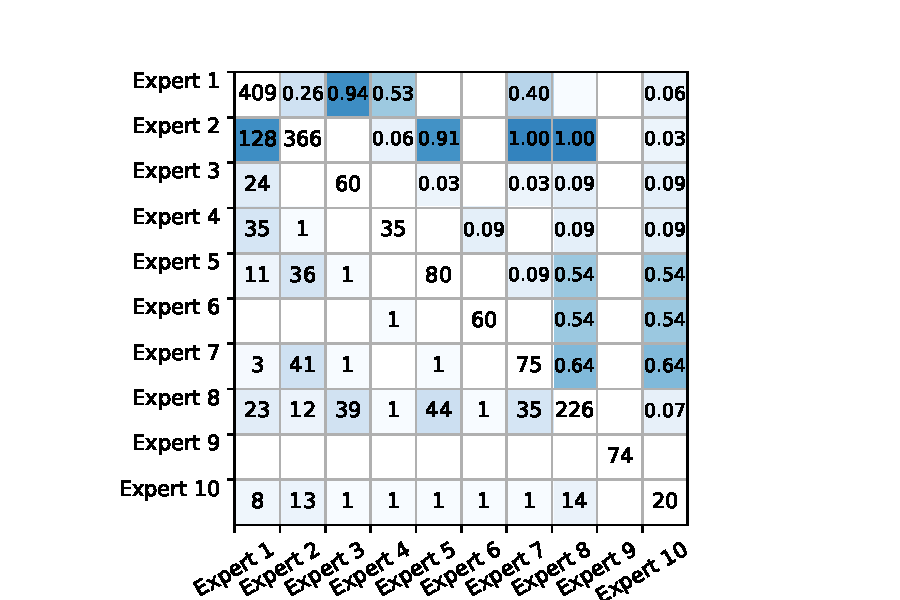
\includegraphics[width=\linewidth]{iaa}
	\caption{$\kappa$ IAA (upper triangular matrix), number of commonly rated triples (lower triangular matrix), and number of ratings (diagonal matrix)}
	\label{fig:iaa}
\end{figure}

\Fref{fig:iaa} shows the $\kappa$ for each pair of experts, as well as the number of overlapping labels. Most triplets (60\%) aren't represented in this figure, since they only received a rating by one expert and very few by more than two. The weighted average of $\overline{k}<0.5$ and few overlapping annotations are not ideal for a reliable development and evaluation of a system. For all experiments each triplet's rounded average rating is considered.

\subsection{Preparing the Dataset}

avg and clip annotator scores, lemmatise sentences, tfidf bow

\section{Ranking Algorithm}

\section{Evaluation and Conclusion}
The system's performance is measured by the Normalised Discounted Cumulative Gain (NDCG). The rank at position $p$ is calculated by
\begin{equation}
NDCG_p = \frac{DCG_p}{IDCG_p},\;
DCG_p = rel_1 + \sum_{i=2}^{p} \frac{rel_i}{\log_2(i+1)}
\end{equation}
where $DCG_p$ is the Discounted Cumulative Gain (DCG) when ordering items based on a given score, $IDCG_p$ the ideal DCG, and $rel_i$ the relevance of an item at position $i$ as depicted by the experts.

\begin{table}
	\caption{Experimental results}
	\label{tab:freq}
	\begin{tabular}{lcc}
		\toprule
		Approach & NDCG & $\sigma ($NDCG$)$\\
		\midrule
		Baseline (random) & $0.87$ & $0.07$\\
		Baseline (worst) & $0.73$ & $0.13$\\
		\bottomrule
	\end{tabular}
\end{table}